\section*{Response to Associate Editor}

\subsection{}
\begin{mdframed}
\begin{quote}
We have received valuable comments from four reviewers. Overall, they consider that the current version contains important contributions. In particular, the paper proposes a retransmission-free reliability architecture for OTFS-based LEO NTN downlinks, combining an MDS/Reed--Solomon diversity transform with ephemeris-driven subchannel reliability prediction and finite-blocklength BLER analysis. The topic is timely and technically interesting, with clear strengths in the algebraic recovery guarantees and in the integration of coding, OTFS, and finite-blocklength analysis. The numerical results are extensive and generally convincing. However, substantial revisions are required. In particular, the paper lacks robustness studies for prediction errors and correlated outages, relies on idealized assumptions regarding Doppler effects and channel estimation, and uses limited baseline methods for comparison. Clearer assumptions on latency, a discussion of implementation complexity, and a clarification of the scope are also needed. Therefore, I recommend a major revision.
\end{quote}
\end{mdframed}

\subsection{Response}

We sincerely thank the Associate Editor for the thorough evaluation and for coordinating the review process. We also appreciate the recognition of the timeliness of the topic, the strengths of the algebraic recovery guarantees, and the breadth of the numerical results. We have carefully addressed all concerns raised by the four reviewers. We have substantially strengthened the revised manuscript to address all six areas identified by the Associate Editor, comprising the following changes:
\begin{enumerate}
\item \textbf{Robustness studies for prediction errors and correlated outages:} (i)~A new analytical subsection, Section~IV-E, models prediction imperfections as a log-normal perturbation on the predicted SNR and derives a closed-form BLER expression in Proposition~\ref{prop:bler_imperfect}, validated through Figs.~\ref{fig:bler_robustness} and~\ref{fig:latency_robustness}; (ii)~a Gaussian copula correlated blockage model in Section~II-A (Eq.~\eqref{eq:corr_matrix_blk}) evaluates the system BLER as a function of spatial correlation $\rho_{\mathrm{blk}}$ in a new simulation figure (Fig.~\ref{fig:bler_correlated_blockage}).

\item \textbf{Idealized assumptions regarding Doppler effects and channel estimation:} (i)~A new SINR impairment model in Section~II-C (Eq.~\eqref{eq:sinr_impairments}) captures fractional Doppler and imperfect channel estimation, with two new curves added to Fig.~\ref{fig:otfs_vs_ofdm} to quantify their impact; (ii)~the dominant feeder-link approximation is validated through a sensitivity analysis in Fig.~\ref{fig:prop1_validation}, with a supporting footnote after Eq.~\eqref{eq:combined_snr_final}; (iii)~a new footnote after Theorem~\ref{thm:fbl_bler} clarifies fading model generality.

\item \textbf{Limited baseline methods for comparison:} (i)~MRC and SC baselines are included in the latency comparison (Fig.~\ref{fig:latency_comparison}) and rate-optimised MRC and SC in the throughput comparison (Fig.~\ref{fig:throughput}); (ii)~a new FEC comparison figure (Fig.~\ref{fig:fec_comparison}) demonstrates FEC-agnostic operation with both polar and LDPC codes at three code rates.

\item \textbf{Clearer assumptions on latency:} (i)~The HARQ-CC baseline is formalised in Section~IV-D with explicit equations for the system BLER (Eq.~\eqref{eq:harq_bler}) and transmission latency (Eq.~\eqref{eq:harq_latency}); (ii)~a new discussion in Section~IV-F addresses inter-subchannel timing advance and block-level synchronisation.

\item \textbf{Implementation complexity:} A new subsection, Section~IV-F, analyses encoding/decoding complexity, transform construction and update overhead, memory footprint, and signalling requirements.

\item \textbf{Clarification of scope:} A new paragraph in Section~IV-F discusses compatibility with the 3GPP NTN framework and confirms that the proposed architecture requires no modification to the satellite payload or UE transmitter.
\end{enumerate}
Below, we provide detailed responses to each of the Associate Editor's six concerns, with supporting manuscript excerpts. Point-by-point responses to each reviewer follow in subsequent sections.

%======================================================================
\subsubsection*{1. Robustness Studies for Prediction Errors and Correlated Outages}
%======================================================================

Two dedicated robustness studies have been added to the revised manuscript.

\vskip 0.1in
\noindent\textbf{1a) Robustness to Prediction Imperfections.}

A new analytical subsection, Section~IV-E, ``Sensitivity to Prediction Imperfections,'' and two new simulation figures (Figs.~\ref{fig:bler_robustness} and~\ref{fig:latency_robustness}) have been added. The combined prediction error from three sources of uncertainty, namely orbital ephemeris errors, UE location uncertainty, and atmospheric model mismatch, is modelled as a log-normal multiplicative perturbation on the predicted end-to-end SNR, and a new Proposition provides the closed-form BLER under imperfect prediction. The results show graceful degradation: at $\sigma_p = 4$~dB the BLER increases by only $0.034$, and the latency advantage over HARQ-CC is preserved with less than a twofold penalty. In the revised manuscript, we now write:

\begin{quote}
``{\color{blue}
The prediction framework in Section~\ref{sec:ephemeris_prediction}
assumes perfect ephemeris knowledge and accurate UE positioning.
In practice, three sources of uncertainty introduce discrepancies
between the predicted and actual subchannel SNRs:
(i)~orbital ephemeris errors, which produce elevation-angle
offsets propagating through the slant-range
and atmospheric-loss models in~\eqref{eq:predicted_path_loss};
(ii)~UE location uncertainty, which introduces additional
elevation-angle error; and
(iii)~atmospheric model mismatch, arising from real-time
variability in tropospheric and ionospheric conditions that
deviates from the statistical models used
in~\eqref{eq:predicted_path_loss}.  The combined prediction error for subchannel~$i$ is represented as $\delta_i \sim \mathcal{N}(0, \sigma_p^2)$, where $\sigma_p$~(dB) characterises the aggregate uncertainty. Incorporating this prediction error, the predicted end-to-end SNR for subchannel~$i$ is modelled using the following log-normal multiplicative perturbation model~\cite{Papoulis2002}:
\begin{equation*}
\check{\gamma}_i^{\mathrm{E2E}} =
\gamma_i^{\mathrm{E2E}} \cdot 10^{\delta_i/10},
\end{equation*}
where $\delta_i$ are assumed mutually independent across subchannels.

Under~\eqref{eq:snr_mismatch}, the erasure declaration and
reliability scoring from Section~\ref{sec:ephemeris_prediction}
operate on the mismatched SNR $\check{\gamma}_i^{\mathrm{E2E}}$
rather than the actual $\gamma_i^{\mathrm{E2E}}$.
This introduces two types of misclassification:
a false erasure, where a reliable subchannel
($\gamma_i^{\mathrm{E2E}} \geq \psi_i$) is declared in outage
because $\check{\gamma}_i^{\mathrm{E2E}} < \psi_i$,
unnecessarily consuming MDS redundancy;
and a missed outage, where a degraded subchannel
($\gamma_i^{\mathrm{E2E}} < \psi_i$) is declared reliable
because $\check{\gamma}_i^{\mathrm{E2E}} \geq \psi_i$,
allowing corrupted soft information to enter the FEC decoder.

\noindent\textbf{Proposition~\ref{prop:bler_imperfect} (BLER Under Imperfect Prediction).}
Under the prediction error model~\eqref{eq:snr_mismatch}
and the dominant feeder-link approximation,
the prediction-error-conditioned BLER for subchannel~$i$ is
\begin{equation*}
\check{\epsilon}_i^{\mathrm{E2E}}(\sigma_p)
= \mathbb{E}_{\delta_i}\!\left[
\Upsilon\!\left(L_i - 1,\;
\frac{\left(\psi_i\cdot 10^{-\delta_i/10}
  - \gamma_{i,0}^{\mathrm{det}}\right)^{+}}
{\hat{\gamma}_{i,\mathrm{NLOS}}}\right)\right],
\end{equation*}
where $(x)^{+} \triangleq \max(x,0)$,
$\psi_i = 2^{R_c} - 1$, and the expectation is over
$\delta_i$.
Setting $\sigma_p = 0$
recovers~\eqref{eq:bler_cdf_combined}.
The system BLER under imperfect prediction follows from
Corollary~\ref{cor:sys_bler_poisson} with
$\epsilon_i^{\mathrm{E2E}}$ replaced by
$\check{\epsilon}_i^{\mathrm{E2E}}(\sigma_p)$:
\begin{equation*}
\check{\epsilon}_{\mathrm{sys}}(\sigma_p)
\approx \sum_{j=f_{\max}+1}^{n}
\tilde{P}(F = j;\,\sigma_p),
\end{equation*}
where $\tilde{P}(F = j;\,\sigma_p)$ is evaluated via the
Poisson binomial recursion~\eqref{eq:poisson_binom_recursive}
with parameters
$\{\check{\epsilon}_i^{\mathrm{E2E}}(\sigma_p)\}_{i=1}^{n}$.

\begin{IEEEproof}
{\color{blue}See Appendix~\ref{app:proof_bler_imperfect}.}
\end{IEEEproof}

The resulting impact of prediction imperfections on transmission latency
follows directly from
Corollary~\ref{cor:latency_reduction}.
Under imperfect prediction, the relaxed per-subchannel
target $\check{\epsilon}^{*}(\sigma_p)$ is obtained by
inverting~\eqref{eq:sys_bler_imperfect}:
\begin{equation*}
\sum_{j=f_{\max}+1}^{n}
\tilde{P}(F=j;\,\sigma_p)\big|_{\check{\epsilon}_i^{\mathrm{E2E}}
= \tilde{\epsilon}^{*}\;,\forall\, i}
= \epsilon_{\mathrm{sys}}^{\mathrm{target}}.
\end{equation*}
Since prediction uncertainty generally increases the effective per-subchannel failure probability, i.e.,
$\check{\epsilon}_i^{\mathrm{E2E}}(\sigma_p) \geq
\epsilon_i^{\mathrm{E2E}}$, the relaxed target satisfies
$\check{\epsilon}^{*}(\sigma_p) \leq \epsilon^{*}$,
and the minimum blocklength
from~\eqref{eq:min_blocklength_div} increases to
\begin{equation*}
\check{n}_c^{*}(\sigma_p)
= \frac{V(\gamma)\bigl[Q^{-1}
(\check{\epsilon}^{*}(\sigma_p))\bigr]^2}
{(C(\gamma) - R_c)^2}
\geq n_c^{*}(\epsilon^{*}, \gamma),
\end{equation*}
yielding a corresponding increase in the frame duration
$\check{T}_{\mathrm{frame}}(\sigma_p) =
\check{n}_c^{*}(\sigma_p)/(M_{\mathrm{D}}\Delta f)$.
}% end blue''
\end{quote}

The following discussion has been added to Section~V:

\begin{quote}
``{\color{blue}Fig.~\ref{fig:bler_robustness} evaluates the robustness of the
proposed diversity transform under imperfect subchannel reliability prediction, as
characterised by Proposition~\ref{prop:bler_imperfect}.
The prediction-error standard deviation $\sigma_p$ is
swept from $0$~dB (perfect prediction) to $4$~dB, spanning
the range of realistic mismatch from ephemeris error, UE
location uncertainty, and atmospheric model deviation.
The system BLER degrades gracefully with increasing $\sigma_p$:
at $P_{\mathrm{total}} = 25$~dBW, the BLER increases from
$0.105$ at $\sigma_p = 0$~dB to $0.139$ at $\sigma_p = 4$~dB,
a modest absolute BLER increase of $0.034$.
All diversity transform curves remain significantly
below the polar (no diversity) baseline across the operating
range, confirming that the MDS redundancy effectively mitigates the increased per-subchannel failure rate from prediction mismatch. The system BLER in~\eqref{eq:sys_bler_imperfect} decays proportionally to $(\check{\epsilon}_i^{\mathrm{E2E}})^{d_{\min}}$, preserving the MDS diversity order $d_{\min}$ regardless of
$\sigma_p$.}
\begin{center}
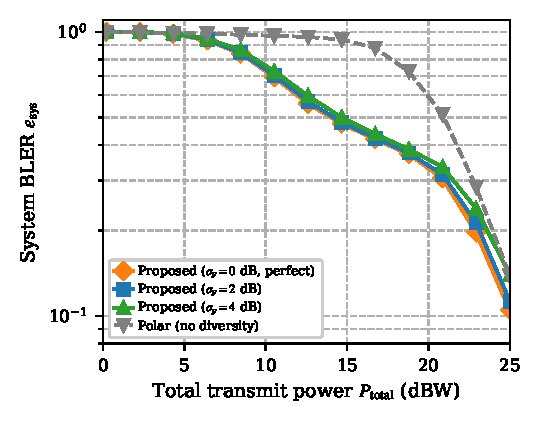
\includegraphics[width=0.7\columnwidth]{bler_robustness_prediction.eps}\\
{\small \textbf{Fig.~\ref{fig:bler_robustness}:} {\color{blue}System BLER versus total transmit power under imperfect
prediction with combined prediction error $\sigma_p$.}}
\end{center}
{\color{blue}Fig.~\ref{fig:latency_robustness} shows the corresponding latency
impact of prediction imperfections on transmission at $P_{\mathrm{total}} = 10$~dBW.
The diversity transform with $\sigma_p = 0$--$4$~dB consistently
achieves lower latency than HARQ-CC across all target system BLER
values, confirming that the latency reduction predicted by~\eqref{eq:min_blocklength_imperfect} is preserved under
realistic prediction imperfections.
At $\sigma_p = 4$~dB, the latency penalty relative to perfect
prediction remains modest, with less than a twofold increase at
$\epsilon_{\mathrm{sys}}^{\mathrm{target}} = 10^{-4}$, while
still achieving approximately two times lower latency than
HARQ-CC.
These results demonstrate that the single-shot decoding advantage
enabled by the diversity transform remains robust to prediction mismatch.}''
\end{quote}



\begin{center}
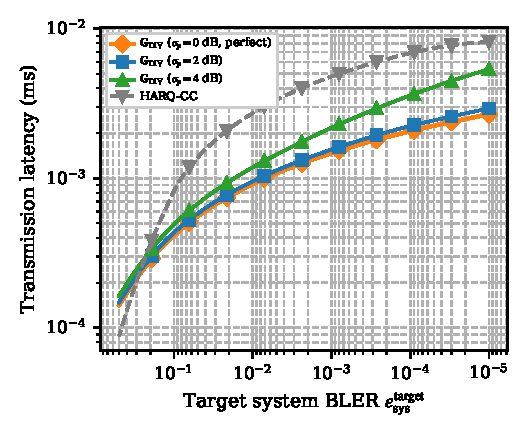
\includegraphics[width=0.7\columnwidth]{latency_robustness_prediction.eps}\\
{\small \textbf{Fig.~\ref{fig:latency_robustness}:} {\color{blue}Transmission latency versus target system BLER under
imperfect prediction at $P_{\mathrm{total}} = 10$~dBW.}}
\end{center}

\vskip 0.1in
\noindent\textbf{1b) Correlated Blockage Model.}

The independent Bernoulli blockage model in Section~II-A has been extended by introducing a Gaussian copula that preserves the elevation-dependent marginal blockage probabilities while introducing pairwise spatial correlation $\rho_{\mathrm{blk}}$ across subchannels. A new figure (Fig.~\ref{fig:bler_correlated_blockage}) evaluates the system BLER as $\rho_{\mathrm{blk}}$ increases from $0$ to $0.9$: the diversity transform maintains the lowest BLER for moderate correlation ($\rho_{\mathrm{blk}} \leq 0.8$), with a crossover near $\rho_{\mathrm{blk}} \approx 0.85$ indicating that the transform should be adaptively bypassed only under near-common blockage. The algebraic recovery guarantee of Theorem~2 holds irrespective of the correlation structure. In the revised manuscript:

\begin{quote}
``{\color{blue}The preceding model treats blockage indicators
$\{B_{i,k\ell}(t)\}$ as independent across subchannels. In practice,
co-visible LEO satellites at similar low elevations share a common
obstruction environment, introducing spatial correlation in blockage
events. To capture this effect, we adopt a Gaussian copula model~{\color{blue}\cite{Nelsen2006, Ghadi2021}}. Let
$\mathbf{Z} = [Z_1, \ldots, Z_n]^\top \sim
\mathcal{N}(\mathbf{0}, \mathbf{R}_{\mathrm{blk}})$,
where the equicorrelation matrix has entries}
\begin{equation*}
\color{blue}
[\mathbf{R}_{\mathrm{blk}}]_{ij} = \begin{cases}
1, & i = j, \\
\rho_{\mathrm{blk}}, & i \neq j,
\end{cases}
\end{equation*}
{\color{blue}with $\rho_{\mathrm{blk}} \in [0,1]$. The blockage indicator of
subchannel~$i$ is then defined as
$B_i = \mathbf{1}\{\Phi(Z_i) \leq P_{\mathrm{LOS}}(\epsilon_i)\}$.
Each subchannel maintains its elevation-dependent marginal
blockage probability
$1 - P_{\mathrm{LOS}}(\epsilon_i)$ from~\eqref{eq:los_prob}, while
$\rho_{\mathrm{blk}}$ controls the degree of spatial correlation:
$\rho_{\mathrm{blk}} = 0$ recovers independent blockage, whereas
$\rho_{\mathrm{blk}} \to 1$ approaches a common-blockage scenario in
which all subchannels tend to be simultaneously obstructed.}''
\end{quote}

The following discussion has been added to Section~V:

\begin{quote}
``{\color{blue}Fig.~\ref{fig:bler_correlated_blockage} evaluates the system
BLER as a function of the blockage correlation parameter
$\rho_{\mathrm{blk}}$ using the Gaussian copula model
in~\eqref{eq:corr_matrix_blk}, with a fixed per-subchannel blockage probability of $0.2$.
At $\rho_{\mathrm{blk}} = 0$, the diversity transform achieves substantially lower BLER than the baselines, consistent with the
independent-blockage results in Fig.~\ref{fig:bler_vs_blockage}.
As $\rho_{\mathrm{blk}}$ increases, the gap narrows because correlated blockage drives the failure
distribution toward two extremes: either all subchannels survive or all are simultaneously blocked. In the former case, the diversity transform
is unnecessary, whereas in the latter, no scheme can recover the data once
more than $f_{\max}$ subchannels are lost.
Consequently, the partial-failure regime, where the MDS recovery
guarantee of Theorem~\ref{thm:block_mds} is most effective, becomes less probable under strong correlation.
For moderate correlation
($\rho_{\mathrm{blk}} \leq 0.8$), the diversity transform
consistently achieves the lowest BLER.
Beyond $\rho_{\mathrm{blk}} \approx 0.85$, however, the baselines
outperform the diversity transform. In this regime, blockage events become nearly common across all subchannels, reducing the benefit of algebraic erasure protection. Consequently, the rate overhead of the MDS diversity
code ($\varrho/n_{\mathrm{out}} = 2/3$) outweighs its recovery gain.
This crossover indicates that the diversity transform is most
effective in the low-to-moderate correlation regime relevant to LEO NTN systems with spatially
separated satellites.  Accordingly, the diversity transform can be adaptively disabled when
the predicted correlation becomes very high $\ldots$}''
\end{quote}

\begin{center}
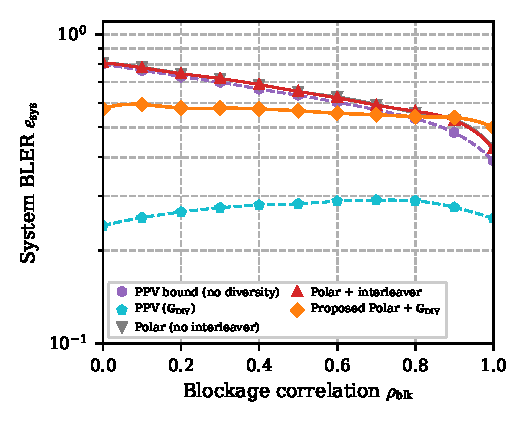
\includegraphics[width=0.7\columnwidth]{bler_vs_correlated_blockage.eps}\\
{\small \textbf{Fig.~\ref{fig:bler_correlated_blockage}:} {\color{blue}System BLER versus blockage correlation
$\rho_{\mathrm{blk}}$ at per-subchannel blockage probability $0.2$.}}
\end{center}

%======================================================================
\subsubsection*{2. Idealized Assumptions Regarding Doppler Effects and Channel Estimation}
%======================================================================

Three aspects of the idealised assumptions have been addressed.

\vskip 0.1in
\noindent\textbf{2a) Fractional Doppler and Imperfect Channel Estimation.}

A new SINR impairment model has been added to Section~II-C that captures both fractional Doppler interference and channel estimation MSE in a single closed-form expression. Two new curves in Fig.~\ref{fig:otfs_vs_ofdm} show that the BLER increases by approximately $1.5$--$2$ times under worst-case fractional Doppler and $-20$~dB channel estimation MSE, yet OTFS remains significantly below OFDM at high normalised Doppler. In the revised manuscript:

\begin{quote}
``{\color{blue}The DD input--output relation in~\eqref{eq:dd_io} assumes
that each tap's Doppler shift aligns exactly with an integer DD bin.
When the physical Doppler $\nu_p$ of the $p$th tap does not coincide
with a grid point, a fractional offset
$\alpha_p = \nu_p - \lfloor\nu_p\rceil$ introduces inter-Doppler
interference with variance
$\sigma_{\mathrm{frac}}^2 = (\pi\,\alpha_p)^2/(3\,N_{\mathrm{D}})$~\cite{Raviteja2018,Moose1994}.
Under imperfect channel estimation with per-element MSE
$\sigma_{\mathrm{CSI}}^2$, the effective post-equalisation SINR is}
\begin{equation*}
\color{blue}
\gamma_i^{\mathrm{eff}} =
\frac{\gamma_i^{\mathrm{c}}}
{1 + \gamma_i^{\mathrm{c}}
\left(\sigma_{\mathrm{frac}}^2
+ \sigma_{\mathrm{CSI}}^2\right)}.
\end{equation*}
{\color{blue}Setting $\alpha_p = 0$ and $\sigma_{\mathrm{CSI}}^2 = 0$
recovers the ideal integer-Doppler, perfect-CSI case.}''
\end{quote}

The following discussion has been added to Section~V:

\begin{quote}
``{\color{blue}To quantify the impact of fractional Doppler and imperfect
channel estimation, Fig.~\ref{fig:otfs_vs_ofdm} also includes the
proposed OTFS scheme under two additional impairment conditions:
(i)~fractional Doppler with worst-case offset $\alpha_p = 0.5$ and perfect channel estimation; and
(ii)~fractional Doppler combined with imperfect channel estimation
($\sigma_{\mathrm{CSI}}^2 = 0.01$, corresponding to a channel estimation MSE of $-20$~dB, which is representative of embedded pilot-aided OTFS estimation at moderate SNR~\cite{Raviteja2018}).
Both impaired OTFS curves exhibit a moderate BLER increase (approximately
$1.5$--$2$ times) relative to the ideal integer-Doppler case, yet
remain significantly below the OFDM curves at high normalised Doppler.
This confirms that the OTFS advantage over OFDM is preserved under
realistic impairments, and that the diversity transform's
subchannel-level recovery guarantee of Theorem~\ref{thm:block_mds}
remains effective.}''
\end{quote}

\begin{center}
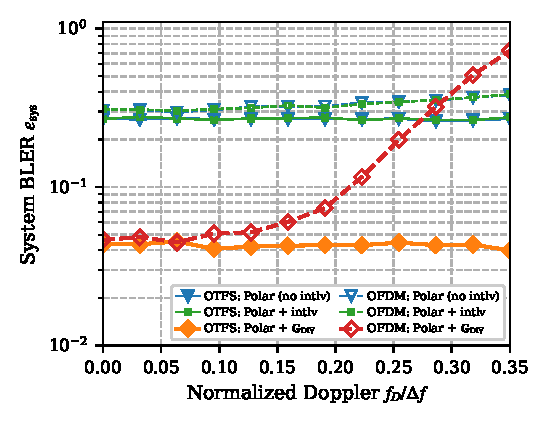
\includegraphics[width=0.7\columnwidth]{otfs_vs_ofdm.eps}\\
{\small \textbf{Fig.~\ref{fig:otfs_vs_ofdm}:} {\color{blue}BLER versus normalised Doppler $f_{D}/\Delta f$ for OTFS
and OFDM at $P_{\mathrm{total}} = 20$~dBW, including fractional
Doppler and imperfect channel estimation impairments.}}
\end{center}

\vskip 0.1in
\noindent\textbf{2b) Dominant Feeder-Link Approximation.}

A footnote after Eq.~(16) in Section~II-B now quantifies the applicability range, and two sensitivity curves have been added to Fig.~\ref{fig:prop1_validation} showing that the BLER loss is less than 1.5~dB when the feeder-to-access margin exceeds 10~dB. The footnote reads:

\begin{quote}
``{\color{blue}Under the parameters in Table~\ref{tab:sim_params}, the ratio $\bar{\gamma}_{i,\mathrm{GS}}/\bar{\gamma}_{i,\mathrm{SU}}$ exceeds 39~dB. According to ITU-R P.618~\cite{ITU-R_P618-14}, Ka-band rain attenuation at 99.9\% link availability for mid-latitude gateway sites is typically 5--12~dB, which reduces this margin to approximately 27--34~dB, well above the 10~dB threshold at which the approximation begins to degrade. The sensitivity of the subchannel BLER to reduced $\bar{\gamma}_{i,\mathrm{GS}}/\bar{\gamma}_{i,\mathrm{SU}}$ is quantified in Fig.~\ref{fig:prop1_validation}.}''
\end{quote}

The following discussion has been added to Section~V:

\begin{quote}
``{\color{blue}Fig.~\ref{fig:prop1_validation} also evaluates the sensitivity of the subchannel BLER to feeder-link degradation by showing simulation results for $n_c = 256$ with reduced feeder-to-access SNR margins of $\bar{\gamma}_{i,\mathrm{GS}}/\bar{\gamma}_{i,\mathrm{SU}} = 10$~dB and $3$~dB, corresponding to severe and extreme Ka-band rain fade conditions, respectively. The BLER loss is less than 1.5~dB when $\bar{\gamma}_{i,\mathrm{GS}}/\bar{\gamma}_{i,\mathrm{SU}}$ exceeds 10~dB, while significant degradation appears only when $\bar{\gamma}_{i,\mathrm{GS}}/\bar{\gamma}_{i,\mathrm{SU}}$ falls below 10~dB, a regime that corresponds to rain attenuation exceeding 30~dB and is typically mitigated through gateway diversity in operational systems.}''
\end{quote}

\begin{center}
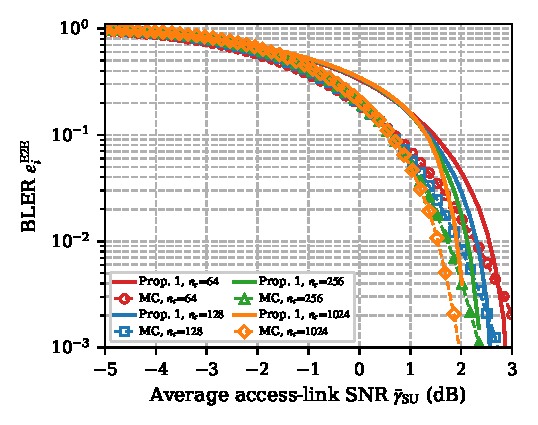
\includegraphics[width=0.7\columnwidth]{prop1_closedform_validation.eps}\\
{\small \textbf{Fig.~\ref{fig:prop1_validation}:} Subchannel BLER versus average access-link SNR for different blocklengths $n_c$ under dominant-LOS Rician fading. {\color{blue}Feeder-link sensitivity is shown for $n_c = 256$ with $\bar{\gamma}_{i,\mathrm{GS}}/\bar{\gamma}_{i,\mathrm{SU}} = 10$~dB and $3$~dB.}}
\end{center}

\vskip 0.1in
\noindent\textbf{2c) Fading Model Generality.}

A new footnote after Theorem~\ref{thm:fbl_bler} in Section~III-A clarifies that the finite-blocklength BLER framework applies to any fading distribution:

\begin{quote}
``{\color{blue}For Nakagami-$m$ fading, the CDF is the regularised lower incomplete gamma function $\Upsilon(m, \gamma/\bar{\gamma})$, and substituting this CDF into~\eqref{eq:bler_exact} recovers the Nakagami-$m$ FBL BLER directly. The Rician and Nakagami-$m$ distributions are related by $m = (K_{i,k\ell}+1)^2/(2K_{i,k\ell}+1)$; setting $K_{i,k\ell} = 0$ yields Rayleigh fading ($m = 1$), as shown in Corollary~\ref{cor:bler_rayleigh}.}''
\end{quote}

The existing figures validate from Rayleigh ($K = 0$, $m = 1$, Fig.~\ref{fig:prop2_diversity}) to dominant-LOS Rician ($K = 2$, $m \approx 1.8$, Fig.~\ref{fig:prop1_validation}).

%======================================================================
\subsubsection*{3. Limited Baseline Methods for Comparison}
%======================================================================

The baseline set has been substantially expanded.

\vskip 0.1in
\noindent\textbf{3a) MRC and SC Baselines in Latency Comparison.}

MRC and SC baselines have been added to Fig.~\ref{fig:latency_comparison} alongside the existing HARQ-CC baseline. Both schemes repeat the same codeword on every subchannel and therefore require $k_c$ times more channel uses for the same message size. The diversity transform achieves the lowest latency among all four schemes at every operating point---approximately three times lower than HARQ-CC at $P_{\mathrm{total}} = 10$~dBW and $\epsilon_{\mathrm{sys}}^{\mathrm{target}} = 10^{-3}$. The following discussion has been added to Section~V:

\begin{quote}
``Fig.~\ref{fig:latency_comparison} demonstrates the latency advantage of the diversity transform over {\color{blue}MRC, SC, and} the HARQ-CC baseline in~\eqref{eq:harq_bler}--\eqref{eq:harq_latency}{\color{blue}, configured with $K_{\max} = 4$, $T_{\mathrm{RTT}} = 20$~ms~\cite{3GPP38821}, and persistent blockage across retransmission attempts. Latency values are geometric means over channel realisations. MRC combines LLRs from all non-blocked subchannels (effective SNR $= \sum_j \bar{\gamma}_j$), and SC selects the subchannel with the highest instantaneous SNR; both repeat the same codeword on every subchannel and therefore require $k_c$ times more channel uses to deliver the same message size.} Despite the chase combining advantage, the diversity transform consistently achieves lower transmission latency than {\color{blue}all three baselines} across all operating points. {\color{blue}For example, at $P_{\mathrm{total}} = 10$~dBW and $\epsilon_{\mathrm{sys}}^{\mathrm{target}} = 10^{-3}$, the diversity transform achieves approximately three times lower latency than HARQ-CC.} As the target system BLER $\epsilon_{\mathrm{sys}}^{\mathrm{target}}$ becomes stricter, HARQ-CC latency grows faster because each additional retransmission round adds a full round-trip time{\color{blue}, while MRC and SC latency grows because their per-subchannel codeword must be $k_c$ times longer to deliver the same message}.''
\end{quote}

\begin{center}
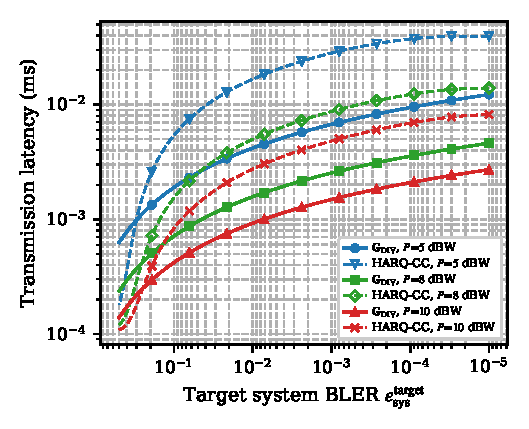
\includegraphics[width=0.7\columnwidth]{latency_comparison.eps}\\
{\small \textbf{Fig.~\ref{fig:latency_comparison}:} {\color{blue}Transmission latency versus target system BLER $\epsilon_{\mathrm{sys}}^{\mathrm{target}}$ for the diversity transform, MRC, SC, and HARQ-CC ($K_{\max} = 4$, $T_{\mathrm{RTT}} = 20$~ms) at $P_{\mathrm{total}} = 5$ and $10$~dBW. MRC and SC require $k_c = 4$ times more channel uses to deliver the same message size.}}
\end{center}

\vskip 0.1in
\noindent\textbf{3b) Rate-Optimised MRC and SC in Throughput Comparison.}

Rate-optimised MRC and SC baselines have been added to Fig.~\ref{fig:throughput}, where the code rate is optimised at each power level to give both schemes their most favourable comparison. Despite this, both saturate at approximately $0.16$~bits per channel use due to the $1/n_{\mathrm{s}}$ repetition penalty, while the diversity transform surpasses MRC at $P_{\mathrm{total}} \approx 12$~dBW and achieves nearly twice the MRC throughput at 25~dBW. The following discussion has been added to Section~V:

\begin{quote}
``{\color{blue}Fig.~\ref{fig:throughput} presents the effective throughput as a function of total transmit power $P_{\mathrm{total}}$ for six schemes. The per-subchannel polar baselines (with and without interleaving) transmit independent data on each subchannel at effective rate $\eta_{\mathrm{eff}} = R_c (1 - \epsilon_{\mathrm{sys}})$, where $R_c = 0.5$. The diversity transform accounts for the MDS rate overhead $\varrho/n_{\mathrm{out}} = 12/18 = 2/3$, yielding $\eta_{\mathrm{eff}} = R_c \cdot (\varrho / n_{\mathrm{out}}) \cdot (1 - \epsilon_{\mathrm{sys}}) \approx 0.33 \cdot (1 - \epsilon_{\mathrm{sys}})$. Rate-optimised MRC and SC are also included. Both schemes repeat the same codeword on all $n_{\mathrm{s}}$ subchannels, giving throughput $\eta_{\mathrm{MRC/SC}} = (R/n_{\mathrm{s}}) \cdot (1 - \epsilon)$, where $R$ is optimised at each operating point to maximise throughput given the combined SNR ($\gamma_{\mathrm{MRC}} = \sum_j \gamma_j$ for MRC, $\gamma_{\mathrm{SC}} = \max_j \gamma_j$ for SC). Despite adaptive rate optimisation, MRC and SC saturate at approximately $0.16$~bits per channel use because of the $1/n_{\mathrm{s}}$ repetition penalty.
Although the diversity transform operates at a lower effective rate than the per-subchannel polar baselines, it achieves higher throughput in the medium-power regime ($6$--$20$~dBW), where the substantial reduction in $\epsilon_{\mathrm{sys}}$ outweighs the MDS rate overhead. The diversity transform surpasses rate-optimised MRC at $P_{\mathrm{total}} \approx 12$~dBW and achieves nearly twice the MRC throughput at $25$~dBW. At high power ($P_{\mathrm{total}} > 22$~dBW), the $\epsilon_{\mathrm{sys}}$ of the per-subchannel polar baselines decreases sufficiently for their higher effective rate ($R_c = 0.5$) to dominate, and their throughput converges with that of the diversity transform.}''
\end{quote}

\begin{center}
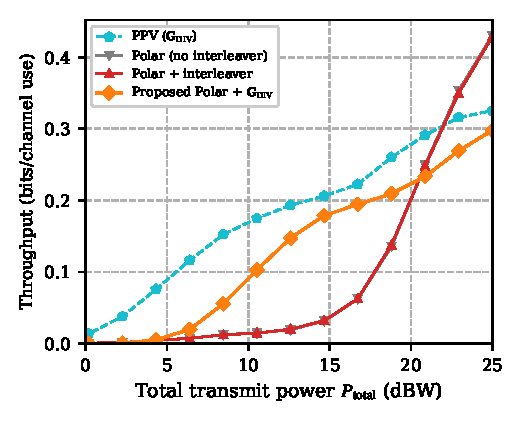
\includegraphics[width=0.7\columnwidth]{throughput_reliability.eps}\\
{\small \textbf{Fig.~\ref{fig:throughput}:} {\color{blue}Effective throughput versus total transmit power at $\epsilon = 40^{\circ}$ with $n_{\mathrm{s}} = 6$ subchannels. The diversity transform operates at effective rate $R_c \cdot \varrho/n_{\mathrm{out}} \approx 0.33$; per-subchannel baselines at $R_c = 0.5$. MRC and SC are rate-optimised at each power level.}}
\end{center}

\vskip 0.1in
\noindent\textbf{3c) FEC-Agnostic Comparison (Polar vs.\ LDPC).}

A new FEC comparison figure (Fig.~\ref{fig:fec_comparison}) has been added to demonstrate that the diversity transform is agnostic to the underlying FEC scheme. Polar codes (SCL decoding, list size~32) and LDPC codes (BP decoding, 50 iterations) are evaluated at three code rates ($R_c \approx 1/4$, $1/2$, $3/4$), and the polar and LDPC curves are nearly indistinguishable (gap $< 0.2$~dB) at every code rate, confirming that the system BLER is dominated by the MDS erasure recovery mechanism. The following discussion has been added to Section~V:

\begin{quote}
``{\color{blue}Fig.~\ref{fig:fec_comparison} demonstrates the FEC-agnostic operation of the proposed diversity transform by comparing polar codes (SCL decoding, list size~$32$) and LDPC codes (BP decoding, $50$ iterations) at three code rates $R_c \approx 1/4$, $1/2$, and $3/4$. All codes are combined with the diversity transform $\mathbf{G}_{\mathrm{DIV}}$ and evaluated under identical channel conditions. At each code rate, the polar and LDPC curves are nearly indistinguishable, with the residual gap remaining below $0.2$~dB across the entire power range. This confirms that the system BLER is dominated by the diversity transform's erasure recovery mechanism rather than by the specific FEC decoder, confirming FEC-agnostic operation. The diversity gain is largest at higher code rates: at $R_c = 3/4$, the no-diversity baseline remains above $0.25$ even at $P_{\mathrm{total}} = 23$~dBW, whereas the diversity-transform-equipped schemes reach $0.03$, because the weaker FEC protection makes the system more reliant on the erasure recovery provided by $\mathbf{G}_{\mathrm{DIV}}$. At $R_c = 1/4$, the stronger FEC narrows the gap, but the diversity transform still provides a consistent advantage across all power levels.}''
\end{quote}

\begin{center}
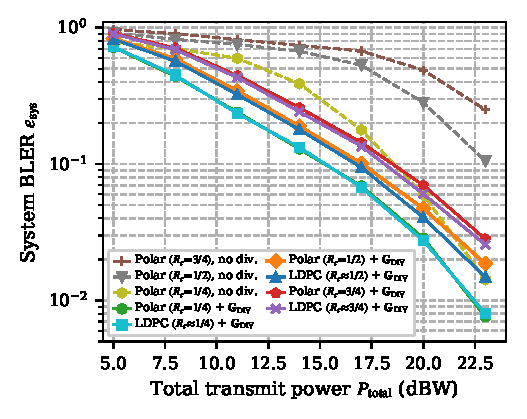
\includegraphics[width=0.7\columnwidth]{fec_comparison.eps}\\
{\small \textbf{Fig.~\ref{fig:fec_comparison}:} {\color{blue}System BLER versus total transmit power for polar and LDPC codes with the proposed diversity transform. No-diversity baselines shown for reference.}}
\end{center}

%======================================================================
\subsubsection*{4. Clearer Assumptions on Latency}
%======================================================================

\noindent\textbf{4a) HARQ-CC Model Formalisation.}

The HARQ-CC baseline has been formalised in Section~IV-D with explicit equations for the system BLER after $K_r+1$ chase combining attempts and the average transmission latency, including the SNR accumulation model and joint optimisation of blocklength and retransmission count. All configuration parameters ($K_{\max} = 4$, $T_{\mathrm{RTT}} = 20$~ms, persistent blockage, geometric mean latency) are now explicitly stated in Section~V:

\begin{quote}
``{\color{blue}For comparison, the conventional HARQ chase combining
(HARQ-CC) baseline operates as follows. After the $k$th
transmission attempt ($k = 0,\ldots,K_{\max}$), the receiver
combines all $k+1$ copies, yielding an effective SNR
$\gamma_{\mathrm{eff}} = \gamma \cdot (k+1)$.
The system BLER after $K_r+1$ attempts is}
\begin{equation*}
\color{blue}
\epsilon_{\mathrm{sys}}^{\mathrm{HARQ}} =
\prod_{k=0}^{K_r} \epsilon\!\left(\gamma(k{+}1),\, n_c,\, R_c\right),
\end{equation*}
{\color{blue}and the average transmission latency is}
\begin{equation*}
\color{blue}
\bar{T}_{\mathrm{HARQ}} = \sum_{k=0}^{K_r} p_k
\left(T_{\mathrm{frame}} + k\,T_{\mathrm{RTT}}\right),
\end{equation*}
{\color{blue}where $p_k$ is the probability of first successful decoding at
attempt~$k$ and $T_{\mathrm{RTT}}$ is the round-trip time.
The blocklength $n_c$ and retransmission count
$K_r \leq K_{\max}$ are jointly optimised to minimise
$\bar{T}_{\mathrm{HARQ}}$ subject to
$\epsilon_{\mathrm{sys}}^{\mathrm{HARQ}} \leq
\epsilon_{\mathrm{sys}}^{\mathrm{target}}$.}''
\end{quote}

All parameters are now explicitly stated: $K_{\max} = 4$, $T_{\mathrm{RTT}} = 20$~ms~\cite{3GPP38821}, persistent blockage across retransmission attempts, and geometric mean latency over channel realisations.

\vskip 0.1in
\noindent\textbf{4b) Inter-Subchannel Timing Advance.}

A new discussion in Section~IV-F addresses block-level synchronisation. The differential propagation delays between the gateway and each satellite are pre-compensated through per-subchannel timing advance, ensuring that all OTFS frames arrive block-aligned at the UE. In the revised manuscript:

\begin{quote}
``{\color{blue}Regarding block-level synchronisation across subchannels, the
diversity transform operates on the algebraic data plane at the
gateway, mapping encoded subwords to transform outputs before
transmission. The differential propagation delays between the
gateway and each satellite are deterministic functions of the
ephemeris-derived slant ranges in~\eqref{eq:slant_range} and are
pre-compensated at the gateway through per-subchannel timing
advance, following the standard 3GPP NTN timing advance
procedure~\cite{3GPP38821}. Consequently, the OTFS frames
arriving at the UE from different satellites are block-aligned,
and the diversity transform construction is independent of the
physical-layer timing.}''
\end{quote}

%======================================================================
\subsubsection*{5. Implementation Complexity}
%======================================================================

A new subsection, Section~IV-F, ``Implementation Complexity,'' has been added to the revised manuscript, covering four aspects: (i) encoding/decoding complexity---the diversity layer adds $O(\varrho \cdot n_{\mathrm{out}} \cdot n_c)$ binary additions, negligible compared to the $O(\varrho \cdot L \cdot N \log N)$ SCL decoding cost; (ii) transform construction---executed once offline with precomputed recovery matrices, requiring only a table index selection per frame; (iii) memory footprint---polynomial in MDS parameters and negligible relative to SCL path storage; and (iv) signalling overhead---at most $\lceil\log_2\binom{n_{\mathrm{s}}}{k_{\mathrm{c}}}\rceil$ bits per frame, or zero if both ends compute the erasure family independently from shared ephemeris data. In the revised manuscript:

\begin{quote}
``{\color{blue}\textbf{Encoding and Decoding Complexity.}
At the transmitter, the diversity mapper computes
$\mathbf{Z} = G_{\mathrm{DIV}}^{\mathsf{T}}\,\mathbf{X}$, where
$\mathbf{X} \in \mathbb{F}_2^{\varrho \times n_c}$ contains the
$\varrho$ polar-encoded subwords. Since $G_{\mathrm{DIV}}$ is binary,
each entry of $\mathbf{Z}$ is obtained by XOR-ing at most $\varrho$
bits, yielding a total of
$O(\varrho \cdot n_{\mathrm{out}} \cdot n_c)$ binary additions.
At the receiver, diversity demapping applies a precomputed binary
recovery matrix
$G_{\mathrm{DIV}}^{\dagger}(E^c) \in
\mathbb{F}_2^{\varrho \times |E^c|}$
at the same asymptotic cost. For $n_c = N$, the diversity layer cost
$O(\varrho\, n_{\mathrm{out}}\, N)$ is typically much smaller than
the total SCL decoding cost $O(\varrho\, L\, N \log N)$, since
$L \log N \gg n_{\mathrm{out}}$ in practical settings. Consequently, the diversity demapping adds negligible
processing latency to the decoding pipeline, preserving the
single-pass receiver architecture described in
Section~\ref{subsec:receiver_demapping}.}

{\color{blue}\textbf{Transform Construction and Update Overhead.}
The RS--Vandermonde construction in
Algorithm~\ref{alg:div_transform_construction} requires
$O(k_{\mathrm{c}} \cdot n_{\mathrm{s}} \cdot m^2)$ finite-field
multiplications to build $G_{\mathrm{MDS}}$ and compute the faithful
binary representation. This computation is executed once offline,
together with all $\binom{n_{\mathrm{s}}}{k_{\mathrm{c}}}$ recovery
matrices, one per admissible erasure pattern, which are stored in a
lookup table.
Since the MDS code parameters $(k_{\mathrm{c}}, n_{\mathrm{s}}, m)$
are fixed for a given system configuration, the matrix
$G_{\mathrm{DIV}}$ itself remains static across frames.
At each frame, the ephemeris-driven predictor in
Section~\ref{sec:ephemeris_prediction} computes per-subchannel
BLER estimates $\tilde{\epsilon}_{i}^{\mathrm{E2E}}$ and
identifies which subchannels exceed the erasure threshold
$\epsilon_{\mathrm{th}}$, producing the predicted outage set
$S_{\mathrm{out}}$ in~\eqref{eq:outage_set}. The receiver then
selects the corresponding precomputed recovery matrix from the
lookup table indexed by $S_{\mathrm{out}}$. Thus, the only
per-frame update is a table index selection, not a matrix
recomputation.}

{\color{blue}\textbf{Memory Footprint.}
The binary diversity transform matrix
$G_{\mathrm{DIV}} \in \mathbb{F}_2^{\varrho \times n_{\mathrm{out}}}$
requires $\varrho \cdot n_{\mathrm{out}}$ bits of storage.
The precomputed recovery matrices, one for each of the
$\binom{n_{\mathrm{s}}}{k_{\mathrm{c}}}$ erasure patterns and
each of size $\varrho \times \varrho$ bits, add
$\binom{n_{\mathrm{s}}}{k_{\mathrm{c}}} \cdot \varrho^2$ bits.
Both quantities scale polynomially in the MDS code parameters and
are negligible compared to the $O(L \cdot N)$ bits required for
SCL decoding path storage.}

{\color{blue}\textbf{Signalling Overhead.}
The diversity transform is determined by the MDS code parameters
$(k_{\mathrm{c}}, n_{\mathrm{s}}, m)$ and the predicted erasure
family $\mathcal{E}_{\mathrm{robust}}$. Since both the gateway
and the UE share ephemeris data
(Section~\ref{sec:ephemeris_prediction}), the erasure family can
be independently computed at both ends without explicit signalling.
In operational scenarios where signalling is preferred for
robustness, the active erasure pattern index requires at most
$\lceil\log_2\binom{n_{\mathrm{s}}}{k_{\mathrm{c}}}\rceil$ bits
per OTFS frame, which is negligible relative to the $n_c$ coded
symbols transmitted per subchannel.}''
\end{quote}

%======================================================================
\subsubsection*{6. Clarification of Scope}
%======================================================================

\noindent\textbf{3GPP NTN Compatibility.}
A new paragraph in Section~IV-F discusses the compatibility of the proposed framework with the 3GPP NTN standard. The diversity transform operates entirely at the gateway side and requires no modification to the satellite payload or UE transmitter. In the revised manuscript:

\begin{quote}
``{\color{blue}From a practical deployment perspective, the proposed diversity transform is compatible with the 3GPP NTN framework. The transform operates entirely at the gateway side, requiring no modification to the satellite payload (which remains a transparent bent-pipe relay) or to the UE physical-layer processing beyond the addition of a soft-decision diversity demapper. The ephemeris-driven prediction relies on satellite orbital data already broadcast in the NR-NTN system information~\cite{3GPP38821}, and the per-subchannel timing advance follows the standard 3GPP NTN procedure. The FEC-agnostic design ensures compatibility with both polar codes (5G NR control channels) and LDPC codes (5G NR data channels), enabling integration into existing NR-NTN protocol stacks without cross-layer redesign.}''
\end{quote}


\vskip 0.2in
We believe that the revisions comprehensively address all six areas identified by the Associate Editor and significantly strengthen the manuscript. We remain committed to providing any additional clarification or revision that may further improve the manuscript. Detailed point-by-point responses to each reviewer follow below.

\newpage